\subsection{Cruces ferroviarios}
    \label{sec:crossing}
    
    Los cruces ferroviarios son la intersección entre la vía ferroviaria y una ruta vehicular o peatonal. Estos cruces pueden ser bajo nivel (túnel por debajo de la vía), sobre nivel (puente vehicular por sobre la vía) o a nivel. Un paso a nivel es una zona muy crítica del sistema ferroviario, ya que, a diferencia de un paso sobre nivel o bajo nivel, conviven simultáneamente la formación y el transito vehicular y peatonal. En la Figura \ref{fig:cruce_1} se ilustra la intersección entre el tendido ferroviario, un cruce vehicular y un cruce peatonal.
    
        \begin{figure}[H]
            \centering
            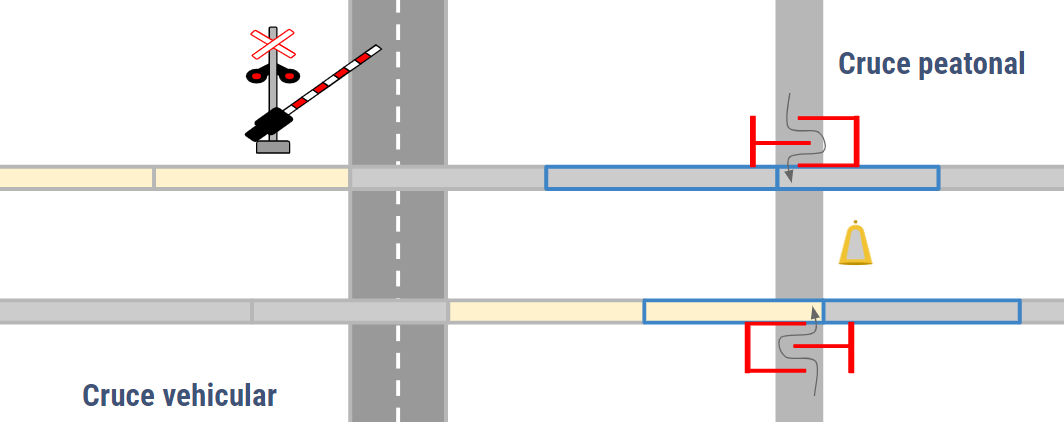
\includegraphics[width=1\textwidth]{Figuras/cruce}
            \centering\caption{Cruces de vías vehiculares y peatonales.}
            \label{fig:cruce_1}
        \end{figure}
        
    Los pasos a nivel peatonales incluyen un pequeño laberinto zigzagueante para forzar al peatón a aminorar su marcha y ver a ambos lados antes de cruzar las vías. A menudo suelen estar acompañados de indicaciones lumínicas y sonoras que se accionan tan pronto el tren se encuentre dentro de un rango de varios metros cercano al paso a nivel, representados por las secciones de via coloreadas en amarillo.
    
    Los pasos a nivel vehiculares añaden barreras ferroviarias para detener el tráfico vehicular cuando un tren se encuentra dentro de un rango de seguridad definido, representados por las secciones de vía coloreadas en rojo.  El sistema de control de la barrera mantiene el brazo de esta en alto para permitir la circulación vehicular. Si un tren es detectado cerca del paso a nivel, se desenergiza la barrera y comienza a descender el brazo por efecto de la gravedad. Solo cuando la barrera baja, el tren tiene permitido avanzar sobre el cruce, siendo el paso a nivel un sector de altísimo riesgo. Al desocuparse las secciones próximas al paso a nivel, la barrera vuelve a energizarse y se sitúa en estado alto nuevamente, a la espera de otro tren para reiniciar el proceso. 
    
    Se debe destacar que el mismo proceso de descenso de la barrera ocurrirá si esta se desenergiza por una falla electromecánica y/o pérdida de alimentación. Es decir, el sistema asumirá el estado más seguro ante cualquiera de los mencionados fallos, siguiendo el principio de falla segura.

    En el Código \ref{lst:crossing_1} se puede ver la implementación de la clase crossing que modela los cruces de vía. Esta clase se encuentra dentro de la clase infrastructure, que a su vez contiene a la clase functionalInfrastructure. La misma incluye atributos como el nombre asignado, si posee o no indicación lumínica o sonora, la dirección de activación y el netElement al que se encuentran asociado, además de su coordenada relativa dentro del netElement.

    \begin{lstlisting}[language = XML, caption = Clase Platform , label = {lst:crossing_1}]
    <levelCrossingsIS>
        <levelCrossingIS id="lcr7" activation="none">
            <name name="Lc01" language="en"/>
            <spotLocation id="lcr7_sloc01" netElementRef="ne1" applicationDirection="both" intrinsicCoord="0.3145"/>
            <designator register="_Example" entry="LEVEL CROSSING Lc01"/>
            <protection barriers="none" lights="none" acoustic="none" hasActiveProtection="true"/>
        </levelCrossingIS>
    </levelCrossingsIS>
    \end{lstlisting}

	Los datos relativos a la características físicas como el largo y el ancho la encontramos dentro de la clase visualization, dentro de la clase infrastructureVisualizations, como se puede ver en el Código \ref{lst:crossing_2}.
	
    \begin{lstlisting}[language = XML, caption = Clase visualization , label = {lst:crossing_2}]
    <spotElementProjection refersToElement="lcr7" id="vis01_sep4">
        <name name="Lc01" language="en"/>
        <coordinate x="-236.364" y="-240.000"/>
    </spotElementProjection>
    \end{lstlisting}

    Conocer las dimensiones del elemento físico que representa esta clase es fundamental a la hora de analizar el impacto de este elemento en la red y donde se deberían asignar las señales ferroviarias.